\documentclass{article}
\usepackage{tikz}
\usepackage[siunitx]{circuitikz}
\usetikzlibrary{calc,positioning,decorations.pathreplacing}
\usepackage[margin=1in,landscape]{geometry}

\begin{document}
\pagestyle{empty}

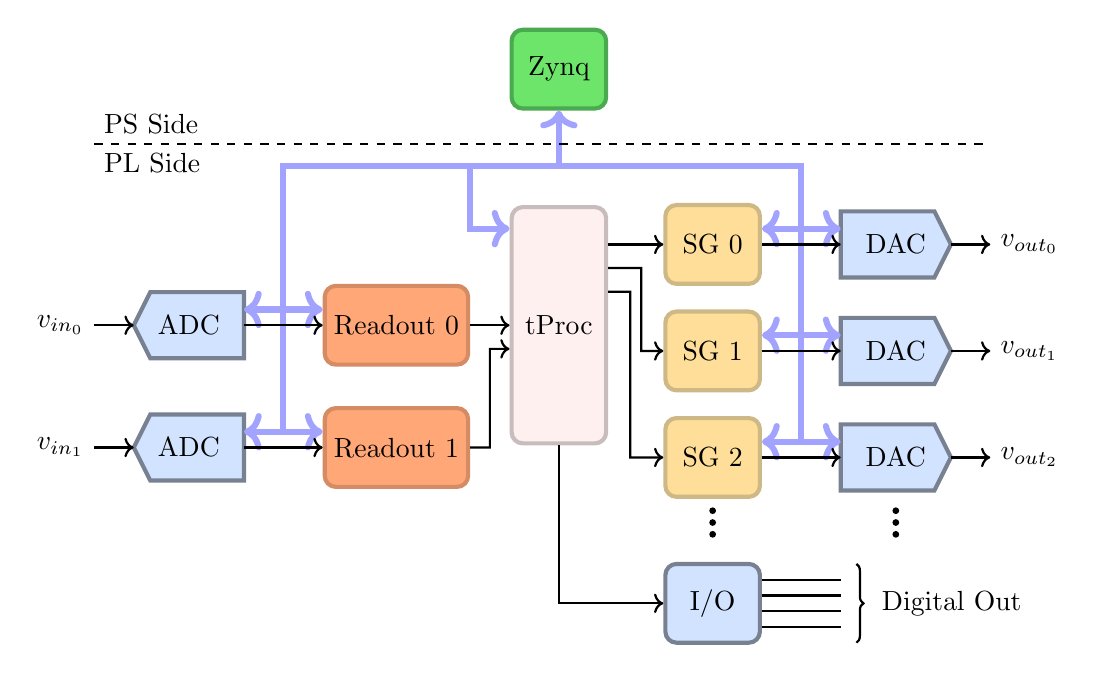
\begin{tikzpicture}
[boxRFSOCproc/.style={align=center, draw,rounded corners,minimum width=1.2cm,minimum height=1cm,draw={rgb,255:red,74; green,170; blue,80},fill={rgb,255:red,109; green,229; blue,107},line width=1.5pt},
boxRFSOCRF/.style={align=center, draw,rounded corners,minimum width=1.2cm,minimum height=1cm,draw={rgb,255:red,120; green,129; blue,145},fill={rgb,255:red,210; green,227; blue,255},line width=1.5pt},
boxSG/.style={align=center, draw,rounded corners,minimum width=1.2cm,minimum height=1cm,draw={rgb,255:red,205; green,184; blue,134},fill={rgb,255:red,254; green,222; blue,152},line width=1.5pt},
boxtProc/.style={align=center, draw,rounded corners,minimum width=1.2cm,minimum height=1cm,draw={rgb,255:red,200; green,188; blue,188},fill={rgb,255:red,255; green,240; blue,240},line width=1.5pt},
boxReadout/.style={align=center, draw,rounded corners,minimum width=1.2cm,minimum height=1cm,draw={rgb,255:red,213; green,139; blue,99},fill={rgb,255:red,255; green,167; blue,118},line width=1.5pt},
arrow/.style={line width=2.2pt,draw={rgb,255:red,162; green,163; blue,255},<->},
single arrow/.style={line width=0.8pt,->},
outmux/.style={muxdemux, muxdemux def={Lh=2,NL=2,Rh=1,NR=1,NB=0,w=1},fill=red!50},
adc/.style={msport,draw={rgb,255:red,120; green,129; blue,145},fill={rgb,255:red,210; green,227; blue,255},line width=0.75pt,circuitikz/RF/scale=2},
node distance=0.5cm]

% tProc.
\node[boxtProc,minimum height=3cm] (tproc) {tProc};

\coordinate (temp) at ($(tproc.north east)+(0.7cm,-0.5)$);

% Signal generators.
\node[boxSG,anchor=west] (sg 0) at (temp) {SG 0};
\node[adc,right=1cm of sg 0,xscale=-1,anchor=right] (dac 0) {};
\node at ($(dac 0.left)!0.5!(dac 0.right)$) {DAC};
\node[boxSG,below=0.3cm of sg 0] (sg 1) {SG 1};
\node[adc,right=1cm of sg 1,xscale=-1,anchor=right] (dac 1) {};
\node at ($(dac 1.left)!0.5!(dac 1.right)$) {DAC};
\node[boxSG,below=0.3cm of sg 1] (sg 2) {SG 2};
\node[adc,right=1cm of sg 2,xscale=-1,anchor=right] (dac 2) {};
\node at ($(dac 2.left)!0.5!(dac 2.right)$) {DAC};
\draw[fill] ($(sg 2.south)+(0,-0.15)$) coordinate (temp) coordinate (temp 1) circle (1pt);
\draw[fill] ($(temp)+(0,-0.15)$) coordinate (temp) circle (1pt);
\draw[fill] ($(temp)+(0,-0.15)$) coordinate (temp) circle (1pt);
\draw[fill] (temp 1 -| dac 2.south) coordinate (temp) circle (1pt);
\draw[fill] ($(temp)+(0,-0.15)$) coordinate (temp) circle (1pt);
\draw[fill] ($(temp)+(0,-0.15)$) coordinate (temp) circle (1pt);

% I/O.
\node[boxRFSOCRF,below=0.8cm of sg 2] (io) {I/O};

% Readout.
\node[boxReadout,left=of tproc] (readout 0) {Readout 0};
\node[adc,left=1cm of readout 0] (adc 0) {ADC};
\node[boxReadout,below=of readout 0] (readout 1) {Readout 1};
\node[adc,left=1cm of readout 1] (adc 1) {ADC};

% Zynq.
\node[boxRFSOCproc,above=1.2cm of tproc] (zynq) {Zynq};

% AXI.
\coordinate (axi start a) at ($(adc 1.right)+(0,0.2)$);
\coordinate (temp) at ($(axi start a)!0.5!(axi start a -| readout 1.west)$);
\coordinate (axi a) at ($(temp |- tproc.north west)+(0,0.5)$);
\coordinate (axi start b) at ($(dac 2.right)+(0,0.2)$);
\coordinate (temp) at ($(axi start b)!0.5!(axi start b -| sg 2.east)$);
\coordinate (axi b) at ($(temp |- tproc.north west)+(0,0.5)$);

\draw[arrow] (axi start a) -- (axi start a -| readout 1.west);
\draw[arrow] ($(adc 0.right)+(0,0.2)$) coordinate (temp) -- (temp -| readout 0.west);
\draw[arrow] (axi start b) -- (axi start b -| sg 2.east);
\draw[arrow] ($(dac 0.right)+(0,0.2)$) coordinate (temp) -- (temp -| sg 0.east);
\draw[arrow] ($(dac 1.right)+(0,0.2)$) coordinate (temp) -- (temp -| sg 1.east);
\draw[arrow,-] (axi start a -| axi a) -- (axi a) -- (axi b) -- (axi b|- axi start b);
\draw[arrow,->] (axi a -| zynq) -- (zynq);
\draw[arrow,->] ($(axi a -| tproc.west)+(-0.5,0)$) |- ($(tproc.north west)+(0,-0.3)$);

% Connections.
\draw[single arrow] (tproc.east |- sg 0) coordinate (temp) -- (sg 0.west);
\draw[single arrow] ($(temp)+(0,-0.3)$) coordinate (temp) -- ($(temp)!0.6!(temp -| sg 0.west)$) |- (sg 1.west);
\draw[single arrow] ($(temp)+(0,-0.3)$) coordinate (temp) -- ($(temp)!0.4!(temp -| sg 0.west)$) |- (sg 2.west);
\draw[single arrow] (tproc.south) |- (io.west);
\draw[single arrow] (readout 0.east) -- (readout 0.east -| tproc.west);
\draw[single arrow] (readout 1.east) coordinate (temp) -- ($(temp)!0.5!(temp -| tproc.west)$) |- ($(tproc.west)+(0,-0.3)$);
\draw[single arrow] (adc 0.right) -- (readout 0);
\draw[single arrow] (adc 1.right) -- (readout 1);
\draw[single arrow] (sg 0.east) -- (dac 0.right);
\draw[single arrow] (sg 1.east) -- (dac 1.right);
\draw[single arrow] (sg 2.east) -- (dac 2.right);

% Vin/vout.
\draw[single arrow,<-] (adc 0.left) -- ++(-0.5,0) node[anchor=east] {$v_{in_0}$} coordinate (vin);
\draw[single arrow,<-] (adc 1.left) -- (adc 1.left -| vin) node[anchor=east] {$v_{in_1}$};
\draw[single arrow] (dac 0.left) -- ++(0.5,0) node[anchor=west] {$v_{out_0}$} coordinate (vout);
\draw[single arrow] (dac 1.left) -- (dac 1.left -| vout) node[anchor=west] {$v_{out_1}$};
\draw[single arrow] (dac 2.left) -- (dac 2.left -| vout) node[anchor=west] {$v_{out_2}$};

% Digital IO.
\draw[single arrow,-] ($(io.east)+(0,0.3)$) -- ++(1,0) coordinate (dout);
\draw[single arrow,-] ($(io.east)+(0,0.1)$) coordinate (temp) -- (temp -| dout);
\draw[single arrow,-] ($(io.east)+(0,-0.1)$) coordinate (temp) -- (temp -| dout);
\draw[single arrow,-] ($(io.east)+(0,-0.3)$) coordinate (temp) -- (temp -| dout) coordinate (dout 1);
\draw[decoration=brace,decorate,thick] ($(dout)+(0.2,0.2)$) -- ($(dout 1)+(0.2,-0.2)$) coordinate (temp);
\node[anchor=west] at ($(temp |- io.west)+(0.2,0)$) {Digital Out};

% PS/PL.
\coordinate (temp) at ($(axi a -| zynq.south)!0.4!(zynq.south)$);
\draw[black!50!black,thick,dashed] (temp -| vin) -- (temp -| vout);
\node[anchor=south west] at (temp -| vin) {PS Side};
\node[anchor=north west] at (temp -| vin) {PL Side};

\end{tikzpicture}

\end{document}
